\documentclass[]{article}
\usepackage[utf8]{inputenc}
\usepackage{polski}
\usepackage{graphicx}
\graphicspath{ {./images/} }
\usepackage[margin=0.5in]{geometry}
\usepackage{gensymb}
\usepackage{textcomp}
\usepackage{siunitx}
\usepackage{float}

\begin{document}

\begin{figure}[tp!]
	\center{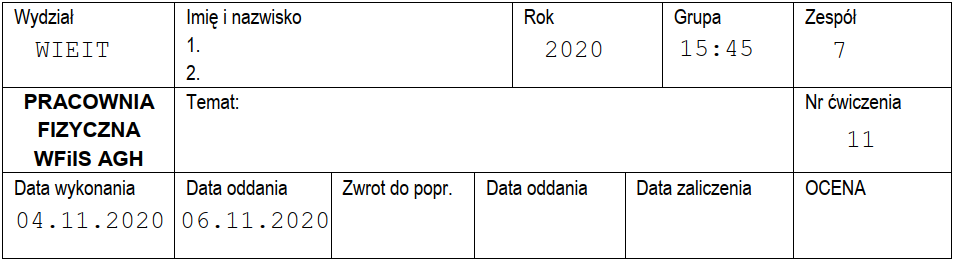
\includegraphics{Name_Card}}
\end{figure}

\begin{center}
	\section*{Moduł Younga}
	\emph{Dzmitry Mikialevich}
\end{center}
\begin{center}
	\emph{Wojciech Sikora}
\end{center}
\tableofcontents
\newpage

\section{Wstęp}

\subsection{Cel ćwiczenia}
Celem doświadczenia jest wyznaczenie modułu Younga metodą statyczną za pomocą pomiaru
wydłużenia drutu z badanego metalu obciążonego stałą siłą.

    
\subsection{Opis ćwiczenia}
Doświadczenie wykonujemy z wykorzystaniem równania prawa Hook'a, określającego proporcjonalność odkształcenia sprężystego do przyłożonej siły:
\newline

\[\Delta l = \frac{Fl}{ES} \]
gdzie E to stała materiałowa czyli mierzony przez nas moduł Younga.
\newline
\newline
Prawo Hooke’a dla rozciągania (lub ściskania) może być też zapisane w postaci wzoru
\[\sigma=E\varepsilon\]
gdzie \(\sigma\) to naprężenie normalne (\(\sigma=\frac{F}{S}\)), a \(\varepsilon\) to normalne odkształcenie względne (\(\varepsilon = \frac{\Delta l}{l}\)).
\newline
\newline
Zgodnie z prawem Hooke'a zależność \(\Delta l (F)\) powinna być prostą \(\Delta l = aF + b\), wobec tego współczynnik \(a = \frac{l}{ES}\). Z tego otrzymujemy:
\[E=\frac{l}{aS}=\frac{4l}{\pi d^2 a}\]

Niepewność złożoną \(u_c(E)\) otrzymujemy:
\[\frac{u_c(E)}{E}=\sqrt{(\frac{u(l)}{l})^2+(-2\frac{u(d)}{d})^2+(-\frac{u(a)}{a})^2}\]
\section{Układ Pomiarowy}
W skład układu pomiarowego weszły następujące elementy:
\newline

1. Przyrząd do pomiaru wydłużenia drutu pod wpływem stałej siły, zaopatrzony w czujnik mikrometryczny do pomiaru wydłużenia drutu.


2. Zestaw odważników


3. Śruba mikrometryczna

4. Przymiar milimetrowy

\begin{figure}[H]
	\center{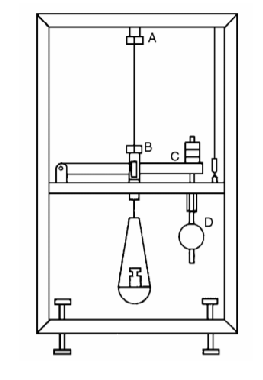
\includegraphics{A}}
	\textbf{\caption{Urządzenie do pomiaru modułu Younga metodą statyczną}}
	
\end{figure}





\section{Przebiegi doświadczenia}
W ramach doświadczenia na początku zmierzyliśmy długość drutu stalowego. Za pomocą śruby mikrometrycznej zmierzyliśmy średnicę drutu, poprzez wykonanie trzech pomiarów w różnych miejscach drutu. Wyzerowaliśmy czujnik mikrometryczny i rozpoczeliśmy pomiary.
\newline
\newline
Badaliśmy wskazania czujnika mikrometrycznego obciążając szalkę odważnikami w zakresie od 0 do 10 kg, zwiększając co 0,5 kg. Następnie zmniejszając obciążenie co 0,5 kg aż do 0 badaliśmy wskazania czujnika.
\newline
\newline
Prawie taką samą procedurę pomiarów dokonaliśmy dla drutu z mosiądzu. Różnica polegała na zakresie od 0 do 6 kg, w gdzie wcześniej było to od 0 do 10 kg.
\newpage
\section{Wyniki Pomiarów}
 Niepewność czujnika przyjęliśmy dla obydwóch przypadków jako 0,01 mm. (Niepewność typu B)
    \subsection{Drut stalowy}
    Długość drutu:\qquad \qquad \qquad \qquad \:\(l = 105,9\: cm \:\:\: u(l) = 1\:mm\)\newline
    Średnica drutu (3 pomiary): \qquad \(d_1 = d_2=d_3 = 0,77\:mm\)\newline
    Średnia średnica:\qquad \qquad \qquad \quad\:\(d_{sr} = 0,77\: mm\) \qquad \(u(d) = 0,01\:mm\)
    

	\begin{table}[h]
		\centering
		\begin{tabular}{|l|l|l|l|l|}
			\hline
Masa odważników [kg] & Czujnik ↑ [mm] & Czujnik ↓ [mm] & Sila F [N] &
\begin{tabular}{@{}c@{}}Wydlużenie średnie\\ \(\) \Delta l \: [mm]\end{tabular} \\ \hline
0,5 & 0,19 & 0,24 & 4,91 & 0,11 \\ \hline
1 & 0,37 & 0,41 & 9,81 & 0,20 \\ \hline
1,5 & 0,51 & 0,60 & 14,72 & 0,28 \\ \hline
2 & 0,67 & 0,78 & 19,62 & 0,36 \\ \hline
2,5 & 0,83 & 0,91 & 24,53 & 0,44 \\ \hline
3 & 0,98 & 1,10 & 29,43 & 0,52 \\ \hline
3,5 & 1,11 & 1,20 & 34,34 & 0,58 \\ \hline
4 & 1,33 & 1,29 & 39,24 & 0,66 \\ \hline
4,5 & 1,47 & 1,48 & 44,15 & 0,74 \\ \hline
5 & 1,62 & 1,65 & 49,05 & 0,82 \\ \hline
5,5 & 1,71 & 1,76 & 53,96 & 0,87 \\ \hline
6 & 1,80 & 1,99 & 58,86 & 0,95 \\ \hline
6,5 & 1,98 & 2,10 & 63,77 & 1,02 \\ \hline
7 & 2,09 & 2,25 & 68,67 & 1,09 \\ \hline
7,5 & 2,35 & 2,35 & 73,58 & 1,18 \\ \hline
8 & 2,48 & 2,51 & 78,48 & 1,25 \\ \hline
8,5 & 2,64 & 2,54 & 83,39 & 1,30 \\ \hline
9 & 2,68 & 2,82 & 88,29 & 1,38 \\ \hline
9,5 & 2,97 & 2,84 & 93,20 & 1,45 \\ \hline
10 & 3,13 & 3,13 & 98,10 & 1,57 \\ \hline
		\end{tabular}
		\textbf{\caption{Wyniki pomiarów dla drutu stalowego}
		}
	\end{table}
\newline
\begin{figure}[H]
	\center{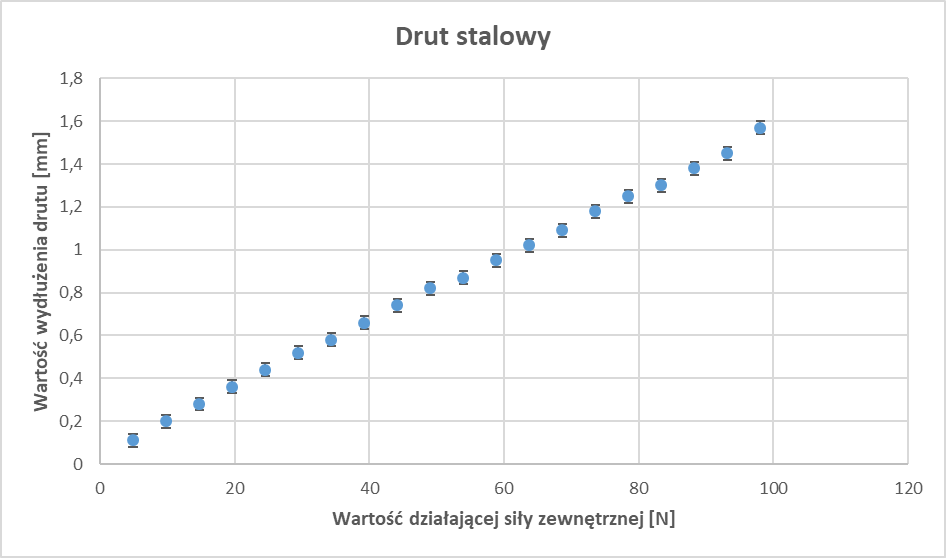
\includegraphics{Graphic1}}
	\textbf{\caption{Wykres otrzymanych wartości wydłużenia drutu w funkcji  działającej siły zewnętrznej}}
\end{figure}

    \subsection{Drut mosiężny}
    Długość drutu:\qquad \qquad \qquad \qquad \:\(l = 106,3\: cm \:\:\: u(l) = 1mm\)\newline
    Średnica drutu (3 pomiary): \qquad \(d_1 = d_2= 1,82\:mm\),\:\:  \(d_3 = 1,85\: mm\)\newline
    Średnia średnica:\qquad \qquad \qquad \quad\:\(d_{sr} = 1,83\: mm\) \qquad \(u(d) = 0,01\:mm\)
    \begin{table}[H]
		\centering
		\begin{tabular}{|l|l|l|l|l|}
			\hline
Masa odważników [kg] & Czujnik ↑ [mm] & Czujnik ↓ [mm] & Sila F [N] &
\begin{tabular}{@{}c@{}}Wydlużenie średnie\\ \(\) \Delta l \: [mm]\end{tabular} \\ \hline
0,5 & 0,27 & 0,31 & 4,91 & 0,15 \\ \hline
1 & 0,55 & 0,58 & 9,81 & 0,28 \\ \hline
1,5 & 0,75 & 0,79 & 14,72 & 0,39 \\ \hline
2 & 1,00 & 0,98 & 19,62 & 0,50 \\ \hline
2,5 & 1,11 & 1,12 & 24,53 & 0,56 \\ \hline
3 & 1,27 & 1,32 & 29,43 & 0,65 \\ \hline
3,5 & 1,37 & 1,43 & 34,34 & 0,70 \\ \hline
4 & 1,54 & 1,64 & 39,24 & 0,80 \\ \hline
4,5 & 1,67 & 1,67 & 44,15 & 0,84 \\ \hline
5 & 1,80 & 1,86 & 49,05 & 0,92 \\ \hline
5,5 & 1,95 & 1,94 & 53,96 & 0,97 \\ \hline
6 & 2,05 & 2,00 & 58,86 & 1,01 \\ \hline

		\end{tabular}
		\textbf{\caption{Wyniki pomiarów dla drutu mosiężnego}
		}
	\end{table}
\begin{figure}[H]
	\center{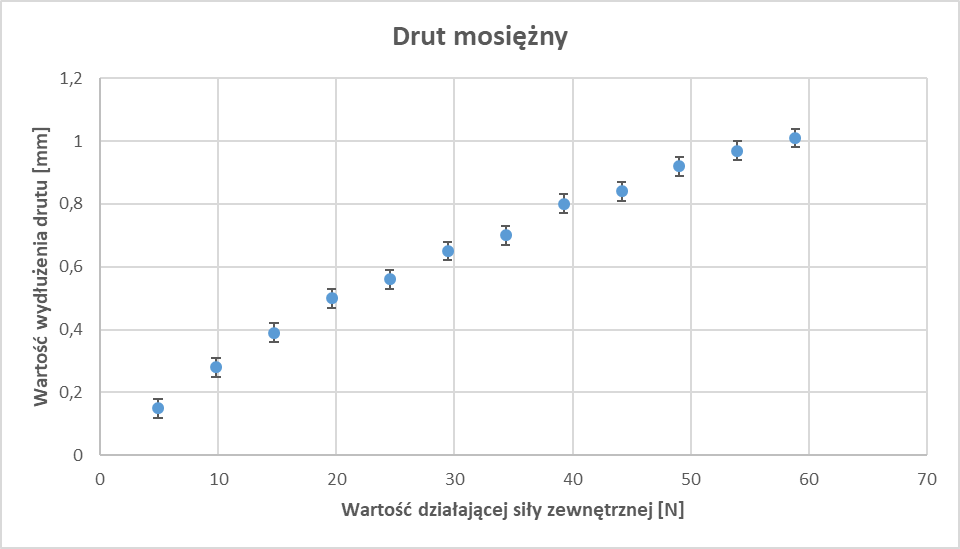
\includegraphics{Graphic2}}
	\textbf{\caption{Wykres otrzymanych wartości wydłużenia drutu w funkcji  działającej siły zewnętrznej}}
\end{figure}
\section{Opracowanie wyników Pomiarów}
    \subsection{Wykresy}
    Za pomocą LINEST w Microsoft Excel obliczyliśmy parametry prostych na Rysunkach 4 i 5 oraz ich niepewności ze współczynnikami korelacji (Tabela 3).\newline
    Tak że ze współczynników korelacji (w obydwóch przypadkach bliskiemu 0) widać, że zależność między wartością działającej siły zewnętrznej a wartością wydłużenia drutu jest liniowa.
\begin{figure}[H]
	\center{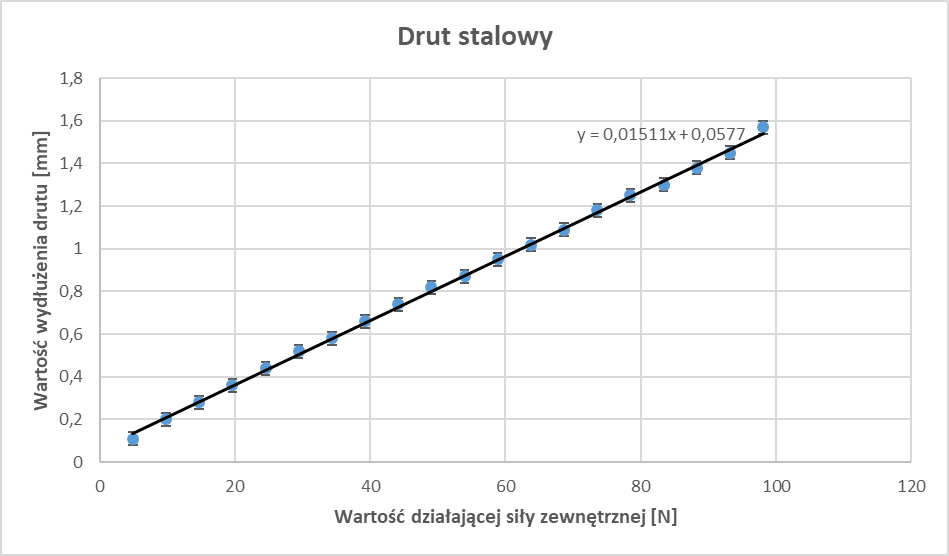
\includegraphics{Graphic3}}
	\textbf{\caption{Wykres otrzymanych wartości \mathbf{v} w funkcji  częstotliwości drgań źródła \mathbf{f}}}
\end{figure}
\begin{figure}[H]
	\center{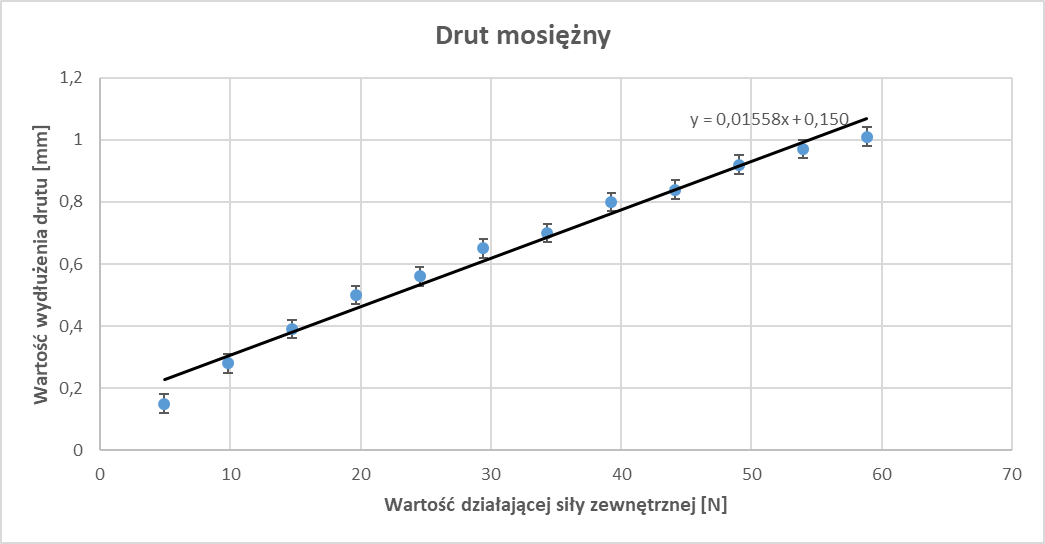
\includegraphics{Graphic4}}
	\textbf{\caption{Wykres otrzymanych wartości \mathbf{v} w funkcji  częstotliwości drgań źródła \mathbf{f}}}
\end{figure}


	\begin{table}[H]
		\centering
		\begin{tabular}{|l|l|l|l|l|l|l|}
			\hline
Drut & 
\begin{tabular}{@{}c@{}}Wartość współczynnika\\ a \: \([\frac{mm}{N}]\) \end{tabular}
 & u(a) [mm]& \begin{tabular}{@{}c@{}}Wartość współczynnika\\ b \: \([\frac{mm}{N}]\) \end{tabular}& u(b) [mm]& \begin{tabular}{@{}c@{}}Wartość współczynnika\\korelacji y \: \([\frac{mm}{N}]\) \end{tabular} & u(y) [mm] \\ \hline
stalowy & 0,01511 & 0,00011 & 0,0577 & 0,0064 & 0,999 & 0,014 \\ \hline
mosiężny & 0,01558 & 0,00069 & 0,150 & 0,024 & 0,980 & 0,040 \\ \hline

		\end{tabular}
		\textbf{\caption{Parametry prostych}
		}
	\end{table}


    \subsection{Obliczanie wartości modułu Younga}
    W celu obliczenia modułu Younga korzystamy z roboczego wzoru:
    \[E=\frac{4l}{\pi d^2 a}\]
    
    
    
    \subsubsection{Wartość modułu Younga dla stalowego drutu}
    Dane pomiarowe z niepewnościami:
    \[a=0,00001511[\frac{m}{N}]\]
    \[u(a)= 0,00000011[\frac{m}{N}]\]
    \[d_s= 0,00077[m]\]
    \[u(d_s)= 0,00001[m]\]
    \[l= 1,059[m]\]
    \[u(l)= 0,001 [m]\]
    
    
\[E=\frac{4l}{\pi d^2 a}=\frac{4*1,059}{3,14*(0,00077)^2*0,00001511} = 150,548953028417\: [GPa] \approx 150,55\:[GPa]\]
    

\[\frac{u(E)}{E}=\sqrt{(\frac{ u(l)}{l})^2+(-2\frac{u(d)}{ d})^2 + (\frac{-u(a)}{a})^2}\]
czyli
\[u(E)=E\sqrt{(\frac{ u(l)}{l})^2+(-2\frac{u(d)}{ d})^2 + (\frac{-u(a)}{a})^2}\]
\[u(E)=150548953028,417\sqrt{(\frac{0,001}{1,059})^2+(-2\frac{0,00001}{ 0,00077})^2 + (\frac{-0,00000011}{0,00001511})^2}= 4,064520139\:[GPa] \approx 4,06\:[GPa]\]


\subsubsection{Wartość modułu Younga dla mosiężnego drutu}
    Dane pomiarowe z niepewnościami:
    \[a= 0,00001558[\frac{m}{N}]\]
    \[u(a)= 0,00000069 [\frac{m}{N}]\]
    \[d_m= 0,00183[m]\]
    \[u(d_m)= 0,00001[m]\]
    \[l= 1,063 [m]\]
    \[u(l)= 0,001[m]\]
    
    
\[E=\frac{4l}{\pi d^2 a}=\frac{4*1,063}{3,14*(0,00183)^2*0,00001558} =25,953382953
\: [GPa] \approx 26,0\:[GPa]\]

    
\[\frac{u(E)}{E}=\sqrt{(\frac{ u(l)}{l})^2+(-2\frac{u(d)}{ d})^2 + (\frac{-u(a)}{a})^2}\]
czyli
\[u(E)=E\sqrt{(\frac{ u(l)}{l})^2+(-2\frac{u(d)}{ d})^2 + (\frac{-u(a)}{a})^2}\]
\[u(E)=25953382953\sqrt{(\frac{0,001}{1,063})^2+(-2\frac{0,00001}{ 0,00183})^2 + (\frac{-0,00000069}{0,00001558})^2}=6,587899787\:[GPa] \approx 6,6\:[GPa]\]


    
  



\subsection{Porównanie z wartościami tablicowymi}


    \begin{table}[H]
		\centering
		\begin{tabular}{|l|l|l|l|}
			\hline
Materiał drutu & E - uzyskane [GPa] & Niepewność u(E) [GPa] & Wartość tabelaryczna E [GPa] \\ \hline
stal & 150,55 & 4,06 & 210-220 \\ \hline
mosiądz & 26,0 & 6,6 & 100 \\ \hline
		\end{tabular}
		\textbf{\caption{Porównanie z wartościami tabelarycznymi}
		}
	\end{table}

\newpage
\subsection{Wnioski}
\begin{itemize}
		\item Wyniki pomiarów modułu Younga to 150,55 \(\pm\) 8,12 [GPa] dla drutu stalowego oraz 26,0 \(\pm\) 13,2 [GPa] dla drutu mosiężnego.
		\item  Wyniki pomiarów w znaczący sposób odbiegają od wartości tabelarycznych, mimo uwzględnienia niepewności pomiaru. Prawdpodobnie jest to spowodowane faktem zużycia drutów, które podczas regularnego używania w doświadczeniach, odkształcily się, tracąc swój pierwotny kształt. Sprawia to, że ich rozciagnięcie jest łatwiejsze niż wynikałoby z teoretycznej zależności.
		\item Innnym powodem niedokładności wyników jest to, że w zależności od miejsca ułożenia odważników na szalce wagi czujnik pokazywał inne odchylenia. Ułożenie odważników w centrum nie zawsze było możliwe. 
	\end{itemize}
\end{document}



% ZROBIĆ OBLICZENIA I POROWNANIE DOPRECYZOWAC!!!